\section{Related Work}

In the book Forecasting: Principles and Practice \cite{fpp3} the authors that also significantly advanced the field go over the main parts of creating forecasts. It goes over the core principles that we will be using to create models for our solution. Besides the core principles, it goes over seasonal and trend decomposition using Loess (STL), auto-correlation functions (ACF), evaluation of forecast accuracy, timeseries cross-validation, regression models, exponential smoothing and ARIMA. However, they wrote this book with the intention to give the reader tools to create the best forecasts they can by manually selecting a model, choosing hyper-parameters and evaluate them using error metrics. It does not touch on the topics of AutoML or auto model selection.


\subsection{Forecasting Competitions}

% https://www.sciencedirect.com/science/article/pii/S0169207019301128
The \emph{M4 Competition} \cite{M4}, that started on January 1, 2018, and ended on May 31, 2018, follows the three previous M competitions, the purpose of which was to learn from empirical evidence both how to improve the forecasting accuracy and how such learning could be used to advance the theory and practice of forecasting. The paper analyzes the solutions used by the participants and compares it to several baseline models. Surprisingly, many teams were beaten by baseline methods, which shows that forecasting can be tricky. They also compare the computational time required to create their forecasts and incorporate baseline methods into this graph shown in figure \ref{fig:m4-time-vs-error}.

\begin{figure*}
\centerline{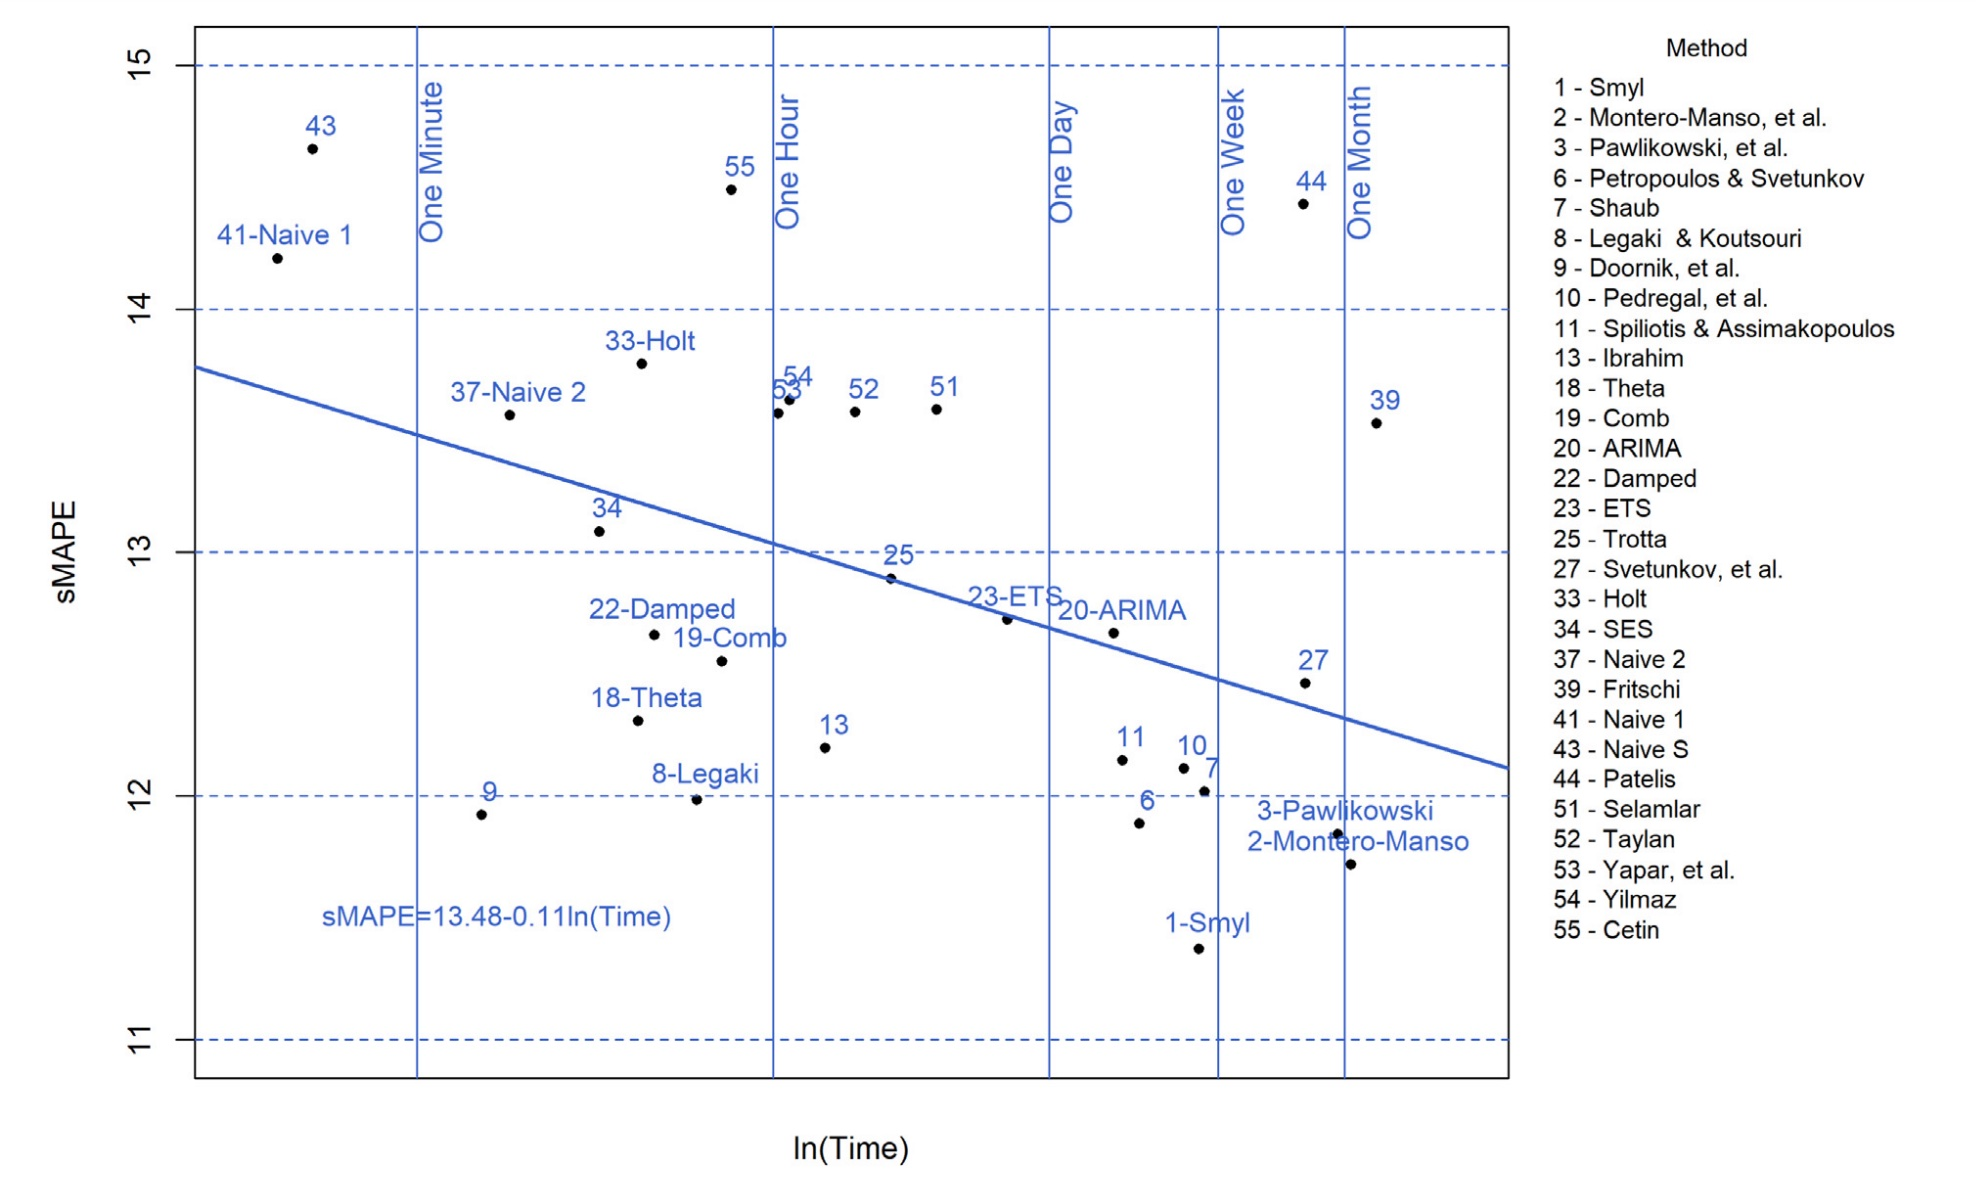
\includegraphics[scale=.25]{Figures/m4-time-vs-error.jpg}}
\caption{Evaluation of the M4 competition's winners \cite{M4}. The plot shows several baseline methods (Naive 1+2, SES, Holt, ETS, Damped, ARIMA, Comb, Theta) as well as the names of the participant groups. The dataset contained 100,000 timeseries from several sources with different resolutions from hourly to yearly that had to be forecasted. We can see that the baselines did reasonably well and outperformed most participants' methods in time.}
\label{fig:m4-time-vs-error}
\end{figure*}

The \emph{M5 competition} \cite{M5}, that started on March 3, 2020, and ended on July 1, 2020, set the competition goal to forecast Walmart sales data for around 42,000 products. The results analysis has not been published yet, but the standing can be viewed on the Kaggle leader board. The upper section of the leader board consists mostly of winners that were using Gradient Boosting machines (GBM) to create the forecasts. Until the results are published, we unfortunately do not know how long those participants let their code fit the data, except for a few ones that took multiple hours or slightly more than a day.

Google has also hosted a forecasting competition with the goal to create forecasts for Web Traffic of around 145,000 Wikipedia articles \cite{web-traffic-competition}. The winners are not required to publish how they achieved their result, however, are encouraged to do so. The first place was achieved by a seq2seq \cite{seq2seq} model. The second place went to a user of XGBoost \cite{xgboost}, a type of GBM.

These competitions lead to greater involvement of the forecasting community and ignited new research to happen. We will evaluate our results and see how they fare among the competition rankings. 

\subsection{Off the Shelf Methods}

% https://arxiv.org/pdf/2005.08067.pdf
Based on the M4 study \cite{M4}, authors of a framework embedded in the library sktime investigated how they can incorporate those results into their library. They used sktime to both replicate and extend key results from the M4 forecasting study. They can largely confirm the results and in both error metrics and time, which means we can assume that these baseline methods are hard to beat in both accuracy and compute time. The implemented framework in sktime, explained in the same paper, also allows us to profit from a coherent and re-usable API to implement a zoo of models to evaluate against our chosen datasets.

A type of model which quickly became popular in 2019 and 2020 was \emph{Prophet}. The authors of the paper \emph{Forecasting at Scale} \cite{prophet} explain the insufficiency of previous forecasting methods by taking an example time series that they recorded and tried fitting the data in an automated setting without changing the default parameters on these data. According to the authors, Prophet can work at scale because its hyper-parameters can be left at their defaults and forecasts are relatively fast and accurate. Out of their research, the authors created an R and Python library that implements the described methods and named it Prophet\footnote{\href{https://facebook.github.io/prophet/}{https://facebook.github.io/prophet/}}. In our work we compare this method to other methods and try to apply it only when it is necessary to do so. Although Prophet is quite efficient, it still requires some compute power to fit a timeseries. It also is regularly outperformed by other methods.

Based on the assumptions that baseline models perform reasonably well and that they satisfy our requirements to fit them to models at scale, without the absolute need of a human analyst, we ask the question if we can design an end-to-end system that automatically suggests the best model given the learning task at hand. Our approach needs to be at least as good as applying Prophet in terms of accuracy and better in terms of compute power required. 



\subsection{Timeseries and AutoML}

PyCaret \cite{PyCaret} is a framework to accomplish their version of AutoML. Currently the library supports classification, regression, clustering, anomaly detection and NLP learning problems. Time series forecasting is not yet in the library, but in the works as their next milestone. PyCaret's approach is to find the best model for a timeseries by fitting and evaluating a collection of models and then tune the \(n\) best models and choose the best one. This approach almost guarantees to find the best model and parameters for that task, which is great. However, fitting several dozen models onto a timeseries and then tuning them is time intensive, even if done in parallel, as PyCaret does out of the box. 

FEDOT \cite{fedot} is a library that also wants to do AutoML, but specifically for timeseries forecasting. It takes a completely different approach than PyCaret, by using evolutionary algorithms to build a pipeline. The methods used by FEDOT are limited to regression-based models. When building a model for a timeseries, the FEDOT method figures out which transformations should be used for a regression step. These input features can be Gaussian filters, smoothing, lagged variables and others. The regressor accepting these values is also selected by evolutionary algorithms. The resulting pipeline works out of the box and achieves great results. However, the fact that it's limited to regression-based models and that the evolutionary algorithm still takes several seconds to find the desired pipeline configuration. This method is interesting, but not something we can apply in our research.

Researchers at Microsoft have shown their approach on how to automatically select a model and its parameters for the narrower case of anomaly detection (AD) in their paper \emph{Automated Model Selection for Time-Series Anomaly Detection} \cite{ms-ad-model-selection}. Their method was evaluated on an internal dataset that was collected in their production. The method first extracts several features of the timeseries and creates a feature vector based on variance, auto-correlation, entropy, seasonal period and several others that are not further specified. They then trained a LightGBM model offline with that data, to be able to classify new timeseries by predicting the best AD model. In their model selection they limited themselves to only three models: SR (Spectral Residual), HBOS (Histogram-based Outlier Score) and SH-ESD (Seasonal Hybrid Extreme Studentized Deviate). This makes training the classifier much easier, since there are less classes, and thus less data needed, as traditionally the number of training data required increases with the amount of classes to predict. Their timeseries data also had human-confirmed labels if a datapoint is an anomaly or not. This makes the task supervised learning and makes evaluating the chosen model slightly easier, as they can collect binary classification metrics such as F1, Precision and Recall which will provide more clear divergence between timeseries and their best model. We will try to replicate a similar approach, but by using forecasters instead of anomaly detector models. We will also try to use more than three models.


\subsection{Timeseries Classification}

In our first approach to find the best model we will use timeseries classification to be able to predict which model to use. There are simple methods such as extracting features and fitting a classifier \cite{tsfresh} which we will try. But there are also more advanced and optimized timeseries classification models such as ROCKET \cite{ROCKET} or MrSEQL \cite{MRSEQL} that we will also evaluate. 
One branch of timeseries classification focuses on timeseries that are based on shapes. A shapelet \cite{SHAPELET} is a timeseries subsequences that is identified as being representative of class membership. Shapelets are a powerful approach for measuring phase-independent similarity between time series; they can occur at any point within a series and offer interpretable results for how matches occur. We will not use shapelets as we find that our metrics based timeseries data will not show patterns of shapes that can be compared among each other. Shapelets can for example classify timeseries that are based on the shape of plant leaves.


\subsection{Anomaly Detection}

As seen above and in several research papers, methods to do anomaly detection are plentiful. Models like HBOS \cite{HBOS}, Spectral Residuals \cite{AD-SR} developed by Microsoft and Google's methods \cite{AD-GOOGLE} likely perform very well on this task. We try to limit ourselves in this work to forecasting models and then do anomaly detection based on these forecasts. This has implications that we might not produce the best anomaly detectors out there. The advantage of forecasting based anomaly detection is that the forecast can be visualized, which can be useful in certain use cases, and then the same forecast is used to decide if a new data point is an anomaly or not. This accomplishes two tasks while fitting only one model. The visualized forecast can be used by humans to easily understand what an anomaly will be and what not, as a simple graph with confidence intervals is easy to explain.

\subsection{Anomaly Detection as a Service}

Corporations such as Google, AWS and Microsoft offer APIs or services to send timeseries data and get anomalies back. This type of API is known as \emph{AD as a service}. These corporations however do not reveal how their methods work as they are a blackbox. All companies have published blog posts or white papers, but they are not enough to be able to fully replicate their system, as they want to keep it proprietary. We will explore how those companies could have built their systems.
